\documentclass[a4paper,11pt]{article}
\usepackage{verbatim}
\usepackage{titlesec}
\usepackage{color}
\usepackage{enumitem}
\usepackage{fancyhdr}
\usepackage{tabularx}
\usepackage{latexsym}
\usepackage{marvosym}
\usepackage[empty]{fullpage}
\usepackage[hidelinks]{hyperref}
\usepackage[normalem]{ulem}
\usepackage[english]{babel}
\usepackage{graphicx}

\input glyphtounicode
\pdfgentounicode=1

\usepackage[default]{sourcesanspro}
\urlstyle{same}

\pagestyle{fancy}
\fancyhf{}

\renewcommand{\headrulewidth}{0in}
\renewcommand{\footrulewidth}{0in}

\setlength{\tabcolsep}{0in}

\addtolength{\oddsidemargin}{-0.5in}
\addtolength{\topmargin}{-0.5in}

\addtolength{\textwidth}{1.0in}
\addtolength{\textheight}{1.0in}

\raggedbottom{}
\raggedright{}

%--------SECTIONING COMMANDS---------
% \titleformat{<command>}
%   [<shape>]{<format>}{<label>}{<sep>}
%     {<before-code>}[<after-code>]

% command is the sectioning command to be redefined
% shape is the style of the font; scshape stands for small caps style
% format is the format to be applied to whole title- label and text; absent here
% label defines the label
% sep is the horizontal separation between label and title body
% before-code is the code to be executed before
% after-code is the code to be executed after

\titleformat{\section}
  {\scshape\large}{}
    {0em}{\color{blue}}[\color{black}\titlerule\vspace{0pt}]
%-------------------------------------


%--------REDEFINITIONS----------------
\renewcommand\labelitemii{$\vcenter{\hbox{\tiny$\bullet$}}$}
\renewcommand{\ULdepth}{2pt}
%-------------------------------------


%--------CUSTOM COMMANDS--------------
%\vspace{} defines a vertical space of given size, modifying this in custom commands can help stretch or shrink resume to remove or add content

% resumeItem renders a bullet point
\newcommand{\resumeItem}[1]{
  \item\small{#1}
}

% commands to start and end itemization of resumeItem, rightmargin set to 0.11in to avoid the overflow of resumetItem beyond whatever resumeItemHeading is being used
\newcommand{\resumeItemListStart}{\begin{itemize}[rightmargin=0.11in]}
\newcommand{\resumeItemListEnd}{\end{itemize}}

% resumeSectionType renders a bolded type to be used under a section, used as skill type here, middle element is used to keep ":"s in the same vertical line
\newcommand{\resumeSectionType}[3]{
  \item\begin{tabular*}{0.96\textwidth}[t]{
    p{0.12\linewidth}p{0.02\linewidth}p{0.81\linewidth}
  }
    \textbf{#1} & #2 & #3
  \end{tabular*}\vspace{-2pt}
}

% resumeTrioHeading renders three elements in three columns with second element being italicized and first element bolded, can be used for projects with three elements
\newcommand{\resumeTrioHeading}[3]{
  \item\small{
    \begin{tabular*}{0.96\textwidth}[t]{
      l@{\extracolsep{\fill}}c@{\extracolsep{\fill}}r
    }
      \textbf{#1} & \textit{#2} & #3
    \end{tabular*}
  }
}

% resumeQuadHeading renders four elements in a two columns with the second row being italicized and first element of first row bolded, can be used for experience and projects with four elements
\newcommand{\resumeQuadHeading}[4]{
  \item
  \begin{tabular*}{0.96\textwidth}[t]{l@{\extracolsep{\fill}}r}
    \textbf{#1} & #2 \\
    \textit{\small#3} & \textit{\small #4} \\
  \end{tabular*}
}

% resumeQuadHeadingChild renders the second row of resumeQuadHeading, can be used for experience if different roles in the same company need to added
\newcommand{\resumeQuadHeadingChild}[2]{
  \item
  \begin{tabular*}{0.96\textwidth}[t]{l@{\extracolsep{\fill}}r}
    \textbf{\small#1} & {\small#2} \\
  \end{tabular*}
}

% commands to start and end itemization of resumeQuadHeading, lefmargin for left indent of 0.15in for resumeItems
\newcommand{\resumeHeadingListStart}{
  \begin{itemize}[leftmargin=0.15in, label={}]
}
\newcommand{\resumeHeadingListEnd}{\end{itemize}}


%-------------------------------------------


\begin{document}


\begin{tabularx}{\linewidth}{@{}m{0.8\textwidth} m{0.2\textwidth}@{}}
{
    \textbf{\Huge Dylan Labatt Randle \vspace{2pt}} \newline
    \href{https://dylanrandle.github.io/}{\uline{Website}} \textbf{·}
    \href{https://linkedin.com/in/dylanrandle}{\uline{LinkedIn}} \textbf{·}
    \href{https://github.com/dylanrandle}{\uline{GitHub}} \textbf{·}
    \href{https://scholar.google.com/citations?user=62z1l9cAAAAJ}{\uline{Scholar}}
    \section{Summary}
    \small{
      Machine learning scientist and leader with 5+ years experience and a proven track record building and deploying AI systems for robotics, computer vision, and natural language processing.
    }
} & 
{
    \hfill
    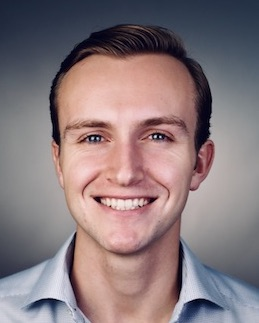
\includegraphics[scale=0.3]{headshot.jpg}
}
\end{tabularx}


\section{Experience}
\resumeHeadingListStart{}
  \resumeQuadHeading{Senior Data Scientist, Machine Learning}{North Reading, MA, USA}
  {Amazon Robotics}{Jul 2020 -- Present}
    \resumeItemListStart{}
      \resumeItem{Led a team of scientists developing AI systems for robotic manipulation and path planning}
      \resumeItem{Delivered performance improvements of +35\% and cost savings of \$10 million/year}
      \resumeItem{Named inventor on two patents}
    \resumeItemListEnd{}
  \resumeQuadHeading{Data Scientist, Machine Learning}{Toronto, ON, Canada}
  {Hubdoc}{Feb 2017 -- Jul 2018}
    \resumeItemListStart{}
        \resumeItem{First machine learning engineer at the startup company (acquired for \$70MM USD)}
        \resumeItem{Developed machine learning system for natural language processing of financial documents}
        \resumeItem{Deployed to production with 99\% precision at 95\% recall, while reducing extraction time by 99.99\%}
    \resumeItemListEnd{}
\resumeHeadingListEnd{}


\section{Education}
  \resumeHeadingListStart{}
    \resumeQuadHeading{Harvard University}{Cambridge, MA, USA}
    {Master of Science in Data Science (GPA: 4.0)}{Aug 2018 -- May 2020}
    \resumeItemListStart{}
      \resumeItem{Thesis: \textit{``Unsupervised Neural Network Methods for Solving Differential Equations"}}
      \resumeItem{Recipient of Scholarship in Applied Computation}
      \resumeItem{Recognized with Distinction in Teaching}
    \resumeItemListEnd{}
    \resumeQuadHeading{University of California, Berkeley}{Berkeley, CA, USA}
    {Bachelor of Science in Industrial Engineering \& Operations Research (GPA: 3.9)}{Aug 2012 -- May 2016}
    \resumeItemListStart{}
      \resumeItem{Recognized with High Honors (\textit{magna cum laude})}
      \resumeItem{Recipient of Frank Kraft Award}
      \resumeItem{Inducted into Phi Beta Kappa, Tau Beta Pi, Alpha Pi Mu}
    \resumeItemListEnd{}
  \resumeHeadingListEnd{}


\section{Sample Projects}
    \resumeItemListStart{}
        \resumeItem{\textbf{Grasp Learning for Robotic Item Manipulation:} Developed ViT and PointNet models for learned grasp generation and ranking. Deployed to production with 36\% reduction in grasp failures.}
        \resumeItem{\textbf{Computer Vision for Robotic Damage Detection:} Developed ResNet-based visual anomaly detection model for damage detection. Achieved +25\% improvement in performance in offline testing.}
        \resumeItem{\textbf{Simulation-Based Optimization for Robotic Path Planning:} Developed simulation-based optimizer for path planning on fleets of thousands of mobile robots. Achieved +10\% improvement in robotic system throughput. Paper published at internal conference.}
        \resumeItem{\textbf{Physics-Informed Neural Networks for Solving Differential Equations:} Developed generative adversarial networks for solving differential equations. Achieved orders of magnitude reduction in solution error over classical approaches. Paper published at ICML 2022 workshop.}
    \resumeItemListEnd{}


\section{Technical Skills}
    \resumeItemListStart{}
        \resumeItem{\textbf{Languages:} Python, C++, Javascript/Typescript, SQL}
        \resumeItem{\textbf{Libraries:} PyTorch, Keras/Tensorflow, OpenCV, Open3D, Pandas, NumPy, SciPy, Scikit-Learn, React}
        \resumeItem{\textbf{Platforms:} AWS, Docker, Firebase, Linux, MacOS}
    \resumeItemListEnd{}


\end{document}